\section{Methodology} \label{sec:methodology}
% detailing the approaches that were used in your experiments; this may also include implementation details in relation to the mobile architecture used
According to \cite{sample_ref}, lorem ipsum dolor sit amet, consetetur sadipscing elitr, sed diam nonumy eirmod tempor invidunt ut labore et dolore magna aliquyam erat, sed diam voluptua. At vero eos et accusam et justo duo dolores et ea rebum. Stet clita kasd gubergren, no sea takimata sanctus est Lorem ipsum dolor sit amet. Lorem ipsum dolor sit amet, consetetur sadipscing elitr, sed diam nonumy eirmod tempor invidunt ut labore et dolore magna aliquyam erat, sed diam voluptua. At vero eos et accusam et justo duo dolores et ea rebum. Stet clita kasd gubergren, no sea takimata sanctus est Lorem ipsum dolor sit amet. Lorem ipsum dolor sit amet, consetetur sadipscing elitr, sed diam nonumy eirmod tempor invidunt ut labore et dolore magna aliquyam erat, sed diam voluptua. At vero eos et accusam et justo duo dolores et ea rebum. Stet clita kasd gubergren, no sea takimata sanctus est Lorem ipsum dolor sit amet.

\subsection{User Journey}
Lorem ipsum dolor sit amet, consetetur sadipscing elitr, sed diam nonumy eirmod tempor invidunt ut labore et dolore magna aliquyam erat, sed diam voluptua. At vero eos et accusam et justo duo dolores et ea rebum.

\subsection{Architecture}

The main goal of the software architecture of soHappy is providing flexibility 
in switching out various components.

Adding a Face- or Smile-Detector based on the technology of liking requires a
developer to implement the designated interface. The implementation can then be 
selected by modifying the configuration file of the app. A configuration-based 
factory will create the Face- or Smile-Detector based on a configuration file. 
(See \ref{fig:arch1})

The Image Analyzer uses the created implementations of Face- and Smile-
Detectors. The results of the Image Analyzer are collected and stored in a
local database.

In order to load and manage the configuration file, an configuration manager 
is used.

\begin{figure}
    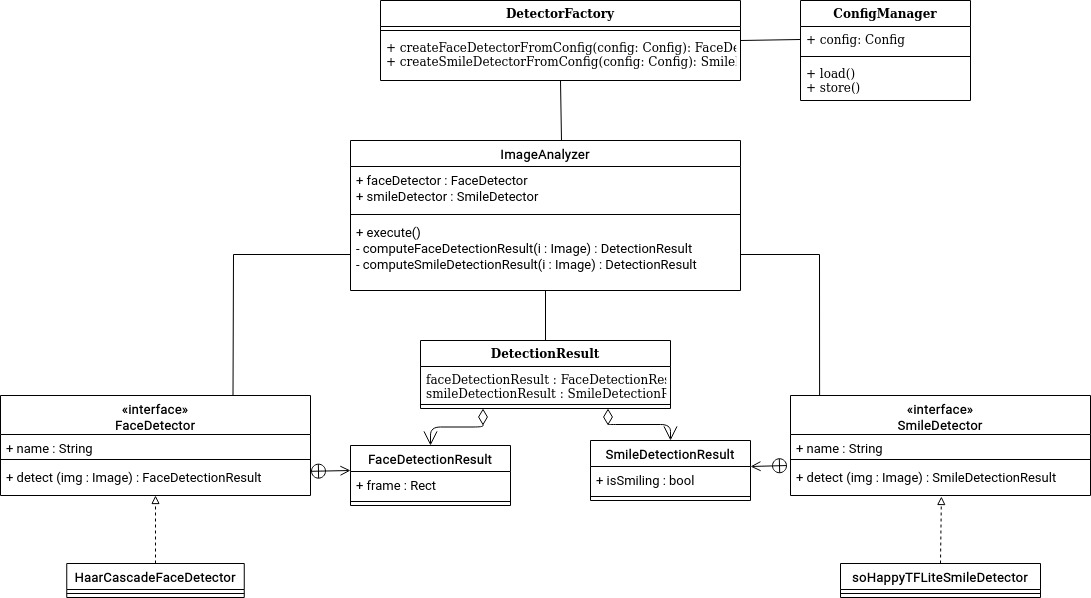
\includegraphics[width=\linewidth]{figures/methodology_architecture_1.jpg}
    \caption{class diagram describing the architecture}
    \label{fig:arch1}
\end{figure}


\subsection{State Machine}
Lorem ipsum dolor sit amet, consetetur sadipscing elitr, sed diam nonumy eirmod tempor invidunt ut labore et dolore magna aliquyam erat, sed diam voluptua. At vero eos et accusam et justo duo dolores et ea rebum.

\subsection{User Interface}
Lorem ipsum dolor sit amet, consetetur sadipscing elitr, sed diam nonumy eirmod tempor invidunt ut labore et dolore magna aliquyam erat, sed diam voluptua. At vero eos et accusam et justo duo dolores et ea rebum.

